\documentclass{article}

\usepackage{graphicx} % Required for inserting images
\usepackage[left=1in,right=1in,top=1in,bottom=1in]{geometry} \usepackage{amsmath}
\usepackage{amsthm} %proof environment
\usepackage{amsthm} %proof environment
\usepackage{amssymb}
\usepackage{amsfonts}
\usepackage{enumitem} %nice lists
\usepackage{verbatim} %useful for something 
\usepackage{xcolor}
\usepackage{setspace}
\usepackage{titlesec}
\usepackage{blindtext} % I have no idea what this is 
\usepackage{caption}  % need this for unnumbered captions/figures
\usepackage{natbib}
\usepackage{appendix}
\usepackage{tikz}
\usepackage{hyperref}

\titleformat{\section}{\bfseries\Large}{Problem \thesection:}{5pt}{}

\begin{document}

\title{AM 260 - Computational Fluid Dynamis: Homework 2}
\author{Dante Buhl}


\newcommand{\wrms}{w_{\text{rms}}}
\newcommand{\bs}[1]{\boldsymbol{#1}}
\newcommand{\tb}[1]{\textbf{#1}}
\newcommand{\bmp}[1]{\begin{minipage}{#1\textwidth}}
\newcommand{\emp}{\end{minipage}}
\newcommand{\R}{\mathbb{R}}
\newcommand{\C}{\mathbb{C}}
\newcommand{\N}{\mathcal{N}}
%\newcommand{\K}{\bs{\mathrm{K}}}
\newcommand{\m}{\bs{\mu}_*}
\newcommand{\s}{\bs{\Sigma}_*}
\newcommand{\dt}{\Delta t}
\newcommand{\dx}{\Delta x}
\newcommand{\tr}[1]{\text{Tr}(#1)}
\newcommand{\Tr}[1]{\text{Tr}(#1)}
\newcommand{\Div}{\nabla \cdot}
\renewcommand{\div}{\nabla \cdot}
\newcommand{\Curl}{\nabla \times}
\newcommand{\Grad}{\nabla}
\newcommand{\grad}{\nabla}
\newcommand{\grads}{\nabla_s}
\newcommand{\gradf}{\nabla_f}
\newcommand{\xs}{x_s}
\newcommand{\x}{\bs{x}}
\newcommand{\xf}{x_f}
\newcommand{\ts}{t_s}
\newcommand{\tf}{t_f}
\newcommand{\pt}{\partial t}
\newcommand{\pz}{\partial z}
\newcommand{\uvec}{\bs{u}}
\newcommand{\bvec}{\bs{B}}
\newcommand{\nvec}{\hat{\bs{n}}}
\newcommand{\tu}{\tilde{\uvec}}
\newcommand{\B}{\bs{B}}
\newcommand{\A}{\bs{A}}
\newcommand{\jvec}{\bs{j}}
\newcommand{\F}{\bs{F}}
\newcommand{\T}{\tilde{T}}
\newcommand{\ez}{\bs{e}_z}
\newcommand{\ex}{\bs{e}_x}
\newcommand{\ey}{\bs{e}_y}
\newcommand{\eo}{\bs{e}_{\bs{\Omega}}}
\newcommand{\ppt}[1]{\frac{\partial #1}{\partial t}}
\newcommand{\pp}[2]{\frac{\partial #1}{\partial #2}}
\newcommand{\pptwo}[2]{\frac{\partial^2 #1}{\partial #2^2}}
\newcommand{\ddtwo}[2]{\frac{d^2 #1}{d #2^2}}
\newcommand{\DDt}[1]{\frac{D #1}{D t}}
\newcommand{\ppts}[1]{\frac{\partial #1}{\partial t_s}}
\newcommand{\pptf}[1]{\frac{\partial #1}{\partial t_f}}
\newcommand{\ppz}[1]{\frac{\partial #1}{\partial z}}
\newcommand{\ddz}[1]{\frac{d #1}{d z}}
\newcommand{\ppzetas}[1]{\frac{\partial^2 #1}{\partial \zeta^2}}
\newcommand{\ppzs}[1]{\frac{\partial #1}{\partial z_s}}
\newcommand{\ppzf}[1]{\frac{\partial #1}{\partial z_f}}
\newcommand{\ppx}[1]{\frac{\partial #1}{\partial x}}
\newcommand{\ddx}[1]{\frac{d #1}{d x}}
\newcommand{\ppxi}[1]{\frac{\partial #1}{\partial x_i}}
\newcommand{\ppxj}[1]{\frac{\partial #1}{\partial x_j}}
\newcommand{\ppy}[1]{\frac{\partial #1}{\partial y}}
\newcommand{\ppzeta}[1]{\frac{\partial #1}{\partial \zeta}}
\renewcommand{\k}{\bs{k}}
\newcommand{\real}[1]{\text{Re}\left[#1\right]}


\maketitle 
% This line removes the automatic indentation on new paragraphs
\setlength{\parindent}{0pt}

\section{Show equivalency between derivations F1-F4}

We will proceed by showing the equivalencies in the following order as
suggested: $(F1) \to (F2) \to (F4) \to (F3) \to (F1)$:

We begin with the first conversion. 

\begin{gather*}
    (F1): \ppt{}\int_V \rho dV = - \int_{\delta V} \rho \uvec \cdot dS\\
    \ppt{}\int_V \rho dV + \int_{V} \grad\cdot \rho \uvec dV = 0\\
    \DDt{}\int_V \rho dV + \int_V \rho \grad\cdot\uvec dV =0\\
    \DDt{}\int_V \rho dV = 0
\end{gather*}
Where here the last term is dropped due to the conversion to the FCV moving with
the flow and no longer remaining stationary. 

The transition from $(F2) \to (F4)$ is much more straightforward. We simply
consider the integral formulation at a very specific control volume such that
the equality must be considered pointwise. 

\begin{gather*}
    \DDt{}\int_{\delta V} \rho dV = \DDt{}\left(\rho \delta V\right ) =
    \DDt{\rho} \delta V + \rho \DDt{\delta V} = \DDt{\rho} + \rho \div{\uvec} =
    0
\end{gather*}

Next we consider the transformation from $(F4) \to (F3)$. We simply have to
simplify the equation in a different way. We have, 
\begin{gather*}
    \DDt{\rho} + \rho \div{\uvec} =  \ppt{\rho} + \uvec\cdot\grad\rho +
    \rho\div{\uvec} = 0\\
    \ppt{\rho} + \div{\rho\uvec} = 0 
\end{gather*}
Thus the conservative and non-conservative forms are exactly the same, simply
expressed algebraically distinctly. Finally, we recover the first expression by
integrating this quantity over some arbitrary control volume. We have, 

\begin{gather*}
    \int_V \ppt{\rho} + \div{\rho\uvec} dV = \int_V \ppt{\rho} dV + \int_{\delta
    V}\rho \uvec \cdot dS\\
    = \ppt{}\int_V \rho dV + \int_{\delta
    V}\rho \uvec \cdot dS
\end{gather*}
where the last step is possible because the FCV does not change in time, only
the density of that FCV. 



\section{Solve the Burgers` equation for the following IC}
\begin{gather*}
    \ppt{u} + \frac{1}{2}\pp{u^2}{x} = 0 \\
    u(x,0) = \begin{cases}
        2, & |x| < 1/2\\
        -1, & |x|  > 1/2
        \end{cases}
\end{gather*}

We solve this using the method of characteristics. 
\begin{gather}
    \ppt{u} + u\ppx{u} = \pp{u}{\tau} = 0\\
    \pp{t}{\tau} = 1, \quad \pp{x}{\tau} = u\\
    t = \tau, \quad x = u\tau + s
\end{gather}

We find that $u$ is constant in $\tau$ or rather time and that the slope of each
characteristic also does not change in time. We notice at there are two discontinuities in the initial condition leading to a
shock wave at $x = 1/2$ and a rarefraction wave originating from $x = -1/2$. We
attempt to find the piecewise solution in the $x-t$ plane for these two
discontinuities. For the shock wave, we look to the Rankine-Hugonoit condition
in order to determine the propagation speed of the shock front. We have, 

\begin{gather*}
    s = \frac{F(u_R) - F(u_L)}{u_R - u_L} = \frac{1/2 - 2}{-1 - 2} = 
    \frac{1}{2}
\end{gather*}

Thus we have that the shock front will have the characteristic defined by $x =
t/2 + \frac{1}{2}$. Next we look to fill in the rarefraction wave using the
notion of self-similarity. That is we center the wave at $x = -1/2$ find the
solution $u$ to be self-similar with respect to $(x+1/2)/t$. We have, 

\begin{gather*}
    u(x,t) = \begin{cases}
                -1 & \text{if } x < -t - \frac{1}{2}\\
                \frac{x+1/2}{t} & \text{if } -t < x+\frac{1}{2} < 2t\\
                2 & \text{if } 2t - \frac{1}{2} < x < \frac{t}{2} + \frac{1}{2}\\
                -1 & \text{if } x > \frac{t}{2} + \frac{1}{2}\end{cases}
\end{gather*}

Notice that the third case for the solution in the $x-t$ plane only exists for a
finite time $t_b$. We solve for this time where the rarefraction wave and shock
front intersect. Specifically we have, 

\begin{gather*}
    2t_b - \frac{1}{2} = \frac{t_b}{2} + \frac{1}{2}\\
    \frac{3}{2}t_b = 1 \implies t_b = \frac{2}{3}
\end{gather*}

A drawing of the characteristics in the $x-t$ plane can be seen in Figure
\ref{fig:p2_drawing}

\begin{figure}[t]
    \centering
    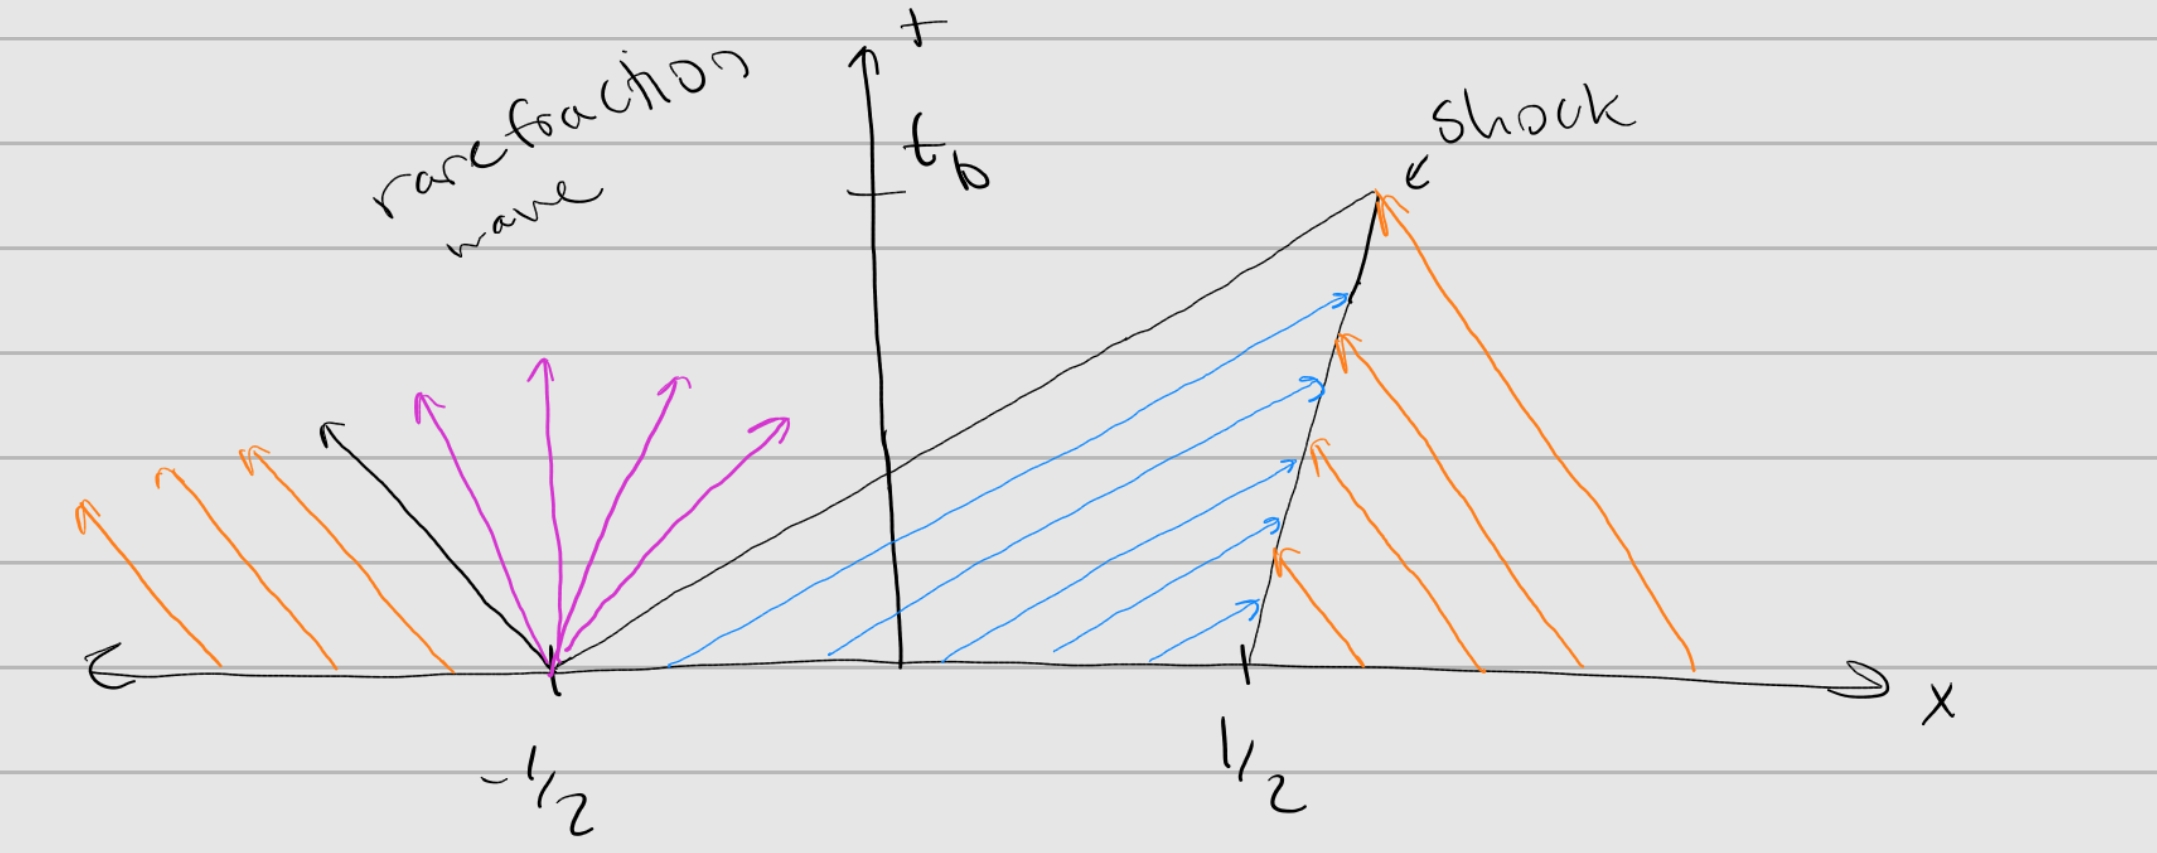
\includegraphics[width=.7\textwidth]{prob2_drawing.jpg}
    \caption{Drawing of the characteristics from problem 2.}
    \label{fig:p2_drawing}
\end{figure}



\section{Solve the scalar conservation law with subsequent IC}
\begin{gather*}
    \ppt{u} + \pp{}{x}\left(\frac{e^u}{2}\right) = 0\\
    u(x,0) = \begin{cases}
        2, & -1 < x < 1\\
        0, & \text{otherwise}
        \end{cases}
\end{gather*}

We begin to solve this problem by determining which type of discontinuity we
have present in the initial condition. We notice that the IC produces values of
$u$ such that at $x = 1$ we have a shock wave, and at $x = -1$ we have a
rarefraction wave. Thus we determine the solution by identifying the shock speed
$s$ and filling in the rarefraction wave. In order to do so we first resolve the
shock. 

\begin{gather*}
    F(u) = F'(u) = \frac{1}{2}e^{u}\\
    s = \frac{F(2) - F(0)}{2 - 0} \approx \frac{3.19}{2} = 1.595
\end{gather*}

We find that the shock propagates with a speed in the x-t plane of 1.595. Note
that with this information we can find the time $t_b$ in which the shock front
intersects with the tail of the rarefraction wave. We have that the shock front
and the right most tail of the rarefraction wave are separated by $\Delta x =
2$. The right tail of the shock has a speed of $c \approx 3.69$. Therefore, we
have,
\begin{gather*}
    3.69t_b = 1.595t_b + 2\\
    t_b = \frac{2}{2.095} \approx 0.954
\end{gather*}

In order to fill in the rarefraction wave, we impose self-similarity
with respect to $(x+1)/t$.

\begin{gather*}
    \frac{e^u}{2} = \frac{x+1}{t}\\
    u = \ln\left(\frac{2(x+1)}{t}\right)\\
    u(x,t) = \begin{cases}
        0 & \text{if } x < \frac{t}{2} - 1\\
        \ln\left(\frac{2(x+1)}{t}\right)& \text{if } \frac{t}{2} < x +1 < \frac{e^2t}{2}\\
        2 & \text{if } \frac{e^2t}{2} - 1 < x < \frac{(e^2-1)t}{4} + 1\\
        0 & \text{if } x > \frac{(e^2-1)t}{4} +1\end{cases}
\end{gather*}

A drawing of the characteristics can be seen in Figure \ref{fig:p3_drawing}
\begin{figure}[t]
    \centering
    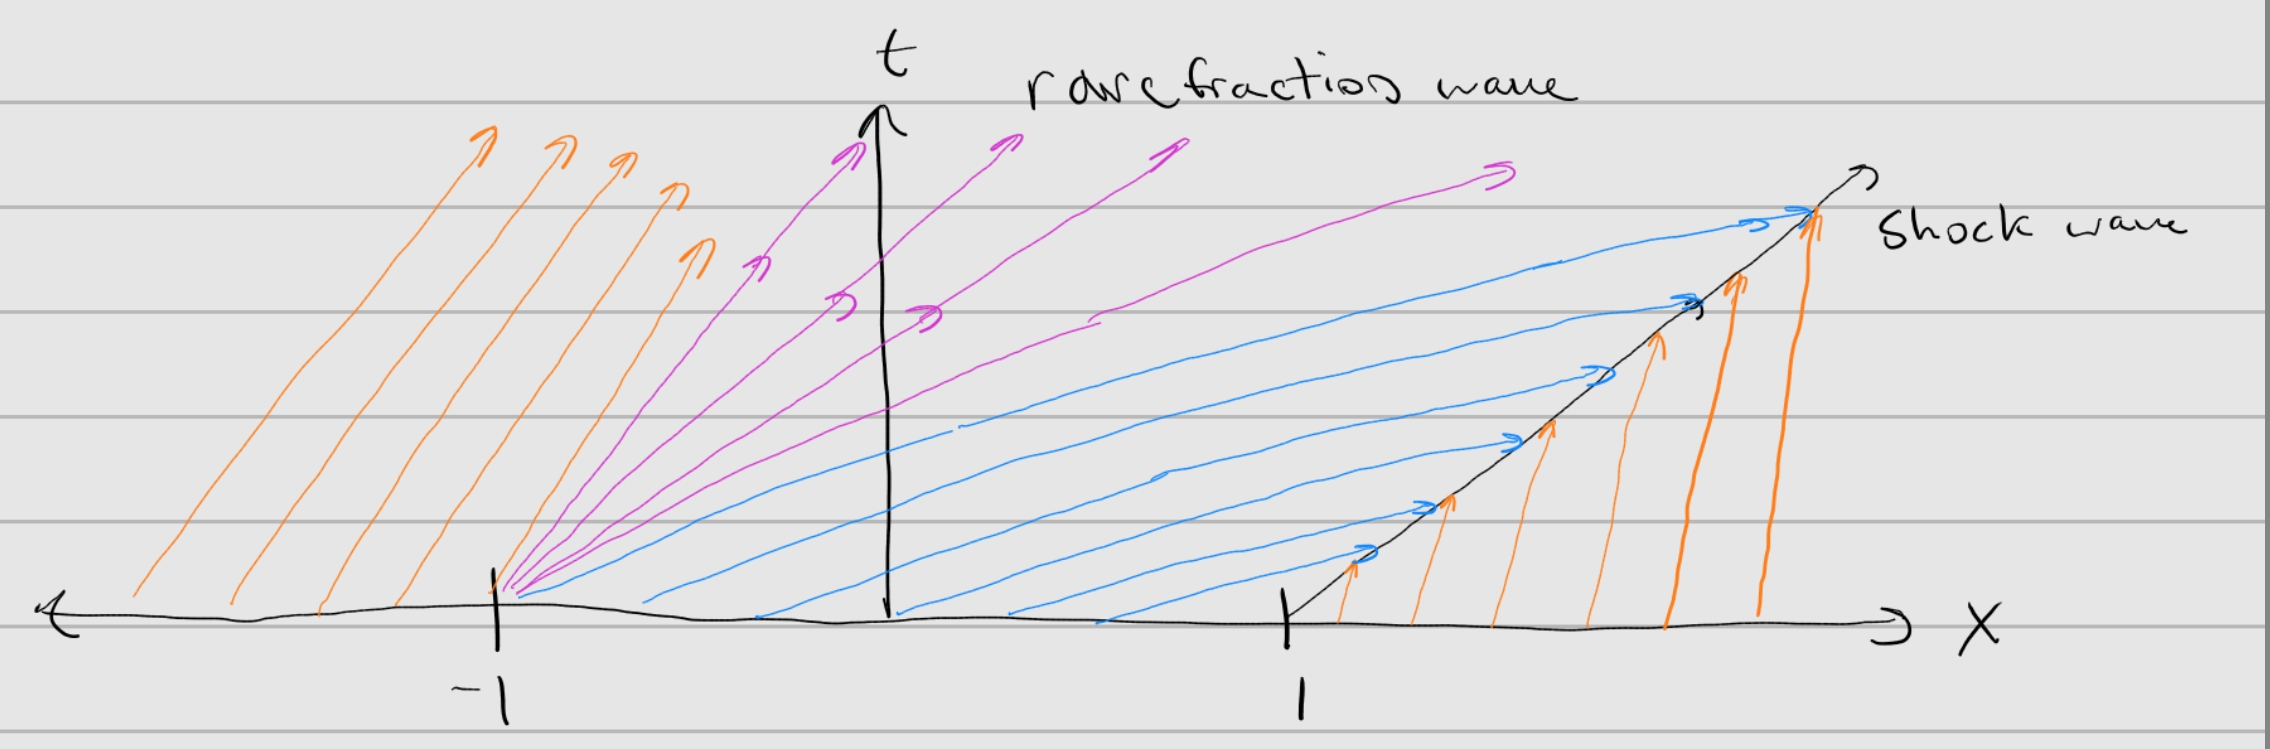
\includegraphics[width=.7\textwidth]{prob3_drawing.jpg}
    \caption{Drawing of the characteristics from problem 3.}
    \label{fig:p3_drawing}
\end{figure}

\section{Weak solutions of the conservation laws}

\textbf{Part A:}

For this section we must show that the the solution, 
\begin{gather*}
    u(x,t) = \begin{cases}
        1 & \text{for } x < t/2\\
        0 & \text{for } x > t/2\end{cases}
\end{gather*}
is a weak solution of the burgers equation. In order to do so, we look at the
definition of a weak solution, i.e. 
\begin{gather*}
    \int_0^{\infty}\int_{-\infty}^{\infty} \ppt{\phi}u +
    \ppx{\phi}f(u) dxdt = -\int_{\infty}^{\infty} \phi(x,0)u(x,0)dx
\end{gather*}

We begin by evaluating the first portion of the integral with integration
by parts. We have, 
\begin{gather*}
    \int\int \phi_t u  dxdt = \int \phi u dx \Big|_0^{\infty} - \int\int \phi
    u_t dxdt
\end{gather*}
After subsituting into the original equation we find, 
\begin{gather*}
    \int \phi u dx \Big|_0^{\infty} +  \int\int - \phi
    u_t + \phi_x f(u)  dxdt \\
    \int \phi u dx \Big|_0^{\infty} +  \int\int \phi
    f_x + \phi_x f  dxdt \\
    \int \phi u dx \Big|_0^{\infty} +  \int\int \ppx{}\left(\phi f\right) dxdt \\
    \int \phi u dx \Big|_0^{\infty} +  \int \phi f\Big|_{-\infty}^{\infty} dt \\
    \int \phi u dx \Big|_0^{\infty} = -\int_{\mathbb{R}} \phi(x,0)u(x,0)dx
\end{gather*}

\textbf{Part B:}

We begin this problem by examining the integral a bit closer. We have, 
\begin{gather*}
    L = \int_a^b u dx = \begin{cases}
        0 & \text{if } \frac{t}{2} < a < b\\
        b - a & \text{if } a < b < \frac{t}{2}\\
        \frac{t}{2} - a & \text{if } a< \frac{t}{2} < b\end{cases}
\end{gather*}
Notice that in only one of these cases does the integral have a non-zerp
derivative in time. We look at this case specifically and evaluate the value of
that time derivative. We have, 
\begin{gather*}
    \ppt{L} = \begin{cases}
        0 & \text{if } \frac{t}{2} < a < b\\
        0  & \text{if } a < b < \frac{t}{2}\\
        \frac{1}{2} & \text{if } a< \frac{t}{2} < b\end{cases}
\end{gather*}
We look then at the specific values for $F(a,t)$ and $F(b,t)$. We have, 
\begin{gather*}
    \left(u(a,t)^2-u(b,t)^2\right)/2 = \begin{cases}
        0  & \text{if } \frac{t}{2} < a < b\\
        0  & \text{if } a < b < \frac{t}{2}\\
        \frac{1}{2} & \text{if } a< \frac{t}{2} < b\end{cases}
\end{gather*}

Therefore we have that the given $u$ satisfies the integral form of the
conservation law. 


\section{Review on WENO and Numerical Methodology (no response required)}

\end{document}
